% ============================================================
%  Graph-Structured Deep Learning for Financial Forecasting
%  Beamer presentation (metropolis theme)
%
%  Build:  pdflatex presentation.tex   (run twice for TOC)
%
%  Figures are pulled directly from the thesis source tree via
%  \graphicspath below — nothing is duplicated.
% ============================================================
\documentclass[aspectratio=169, 10pt]{beamer}

% ---- Theme --------------------------------------------------
\usetheme{metropolis}
\usepackage{appendixnumberbeamer}

% ---- Packages -----------------------------------------------
\usepackage{booktabs}
\usepackage{amsmath, amssymb}
\usepackage{mathtools}
\usepackage{graphicx}
\usepackage{xcolor}
\usepackage{tikz}
\usetikzlibrary{shapes.geometric, arrows.meta, positioning, fit, backgrounds, calc}
\usepackage{pgfplots}
\pgfplotsset{compat=1.18}
\usepackage{multirow}
\usepackage{array}
\usepackage{colortbl}

% ---- Where to find the thesis figures -----------------------
\graphicspath{%
  {../figures/}%
  {../../comparison_results/}%
  {../../stock_analysis_results/}%
  {../../THGNN/data/plots/}%
}

% ---- Colour palette (light-blue scheme) ---------------------
\definecolor{primary}{HTML}{1976D2}
\definecolor{accent}{HTML}{5DADE2}
\definecolor{positive}{HTML}{1E8449}
\definecolor{negative}{HTML}{C0392B}
\definecolor{neutral}{HTML}{7F8C8D}
\definecolor{highlight}{HTML}{F39C12}
\definecolor{lightbg}{HTML}{E3F2FD}
\definecolor{darkbg}{HTML}{1A252F}

\setbeamercolor{palette primary}{bg=primary, fg=white}
\setbeamercolor{frametitle}{bg=primary, fg=white}
\setbeamercolor{progress bar}{fg=accent}
\setbeamercolor{alerted text}{fg=highlight}
\setbeamercolor{block title}{bg=primary, fg=white}
\setbeamercolor{block body}{bg=lightbg}
\setbeamercolor{block title alerted}{bg=negative, fg=white}
\setbeamercolor{block body alerted}{bg=negative!10}

% ---- Global list spacing ------------------------------------
\setlength{\itemsep}{3pt}
\setlength{\parskip}{2pt}

% ---- Custom commands ----------------------------------------
\newcommand{\myvec}[1]{\mathbf{#1}}
\newcommand{\cmark}{\textcolor{positive}{\textbf{\checkmark}}}
\newcommand{\xmark}{\textcolor{negative}{\textbf{\texttimes}}}
\newcommand{\best}[1]{\textcolor{primary}{\textbf{#1}}}

% ---- Metadata -----------------------------------------------
\title{Graph-Structured Deep Learning for Financial Forecasting}
\subtitle{A Hybrid THGNN--MaGNet Architecture and Multi-Agent Decision\\ Pipeline for Indian Equity Markets (NSE)}
\author{Debarshi Chakraborty \quad\textbar\quad ID B2430045}
\date{MSc Big Data Analytics \textbar\ RKMVERI, Belur}
\institute{Supervisor: Mr Champak Kumar Dutta \textbar\ Dept.\ of Computer Science}

% ============================================================
\begin{document}

\maketitle

\begin{frame}{Outline}
  \setbeamertemplate{section in toc}[sections numbered]
  \tableofcontents[hideallsubsections]
\end{frame}

% ============================================================
\section{Motivation \& Problem}
% ============================================================

\begin{frame}{Why Is Financial Forecasting Hard?}
  \begin{columns}[T]
    \begin{column}{0.55\textwidth}
      Stock prices are generated by \alert{millions of interacting agents}
      who observe and anticipate each other.

      \medskip
      \textbf{Consequences for the data:}
      \begin{itemize}\setlength{\itemsep}{3pt}
        \item Non-stationary — structural breaks, regime shifts
        \item \alert{Very low signal-to-noise} — useful rank-IC is only $0.05$--$0.15$
        \item Stocks are \alert{not independent} — sector \& macro shocks couple them
        \item Relationships are \alert{dynamic} — correlations change over time
      \end{itemize}

      \medskip
      \textbf{Two research gaps:}
      \begin{enumerate}\setlength{\itemsep}{2pt}
        \item Most SOTA is tested only on US / Chinese markets — \alert{NIFTY 500 underserved}
        \item Prediction is studied \alert{in isolation} — no end-to-end deployable system
      \end{enumerate}
    \end{column}
    \begin{column}{0.42\textwidth}
      \begin{block}{Task: Cross-Sectional Ranking}
        \textbf{Input:} $\myvec{X}^\tau \in \mathbb{R}^{N \times T \times F}$\\
        \quad $N=353$ NIFTY 500 stocks\\
        \quad $T=20$ trading-day look-back\\
        \quad $F=12$ OHLCV + technical features
        \smallskip\\
        \textbf{Output:} $\hat{\myvec{y}} \in \mathbb{R}^{N}$ — next-day return score
        \smallskip\\
        \textbf{Objective:} maximise rank correlation
        \[ \text{IC} = \text{corr}_\text{Spearman}(\hat{\myvec{y}}, \myvec{y}) \]
      \end{block}
      \footnotesize
      Long top-$K$ / short bottom-$K$: IC directly measures investment value.
    \end{column}
  \end{columns}
\end{frame}

% ============================================================
\section{Background \& Related Work}
% ============================================================

\begin{frame}{The Forecasting Landscape — Two Lineages}
  \begin{columns}[T]
    \begin{column}{0.49\textwidth}
      \textbf{\textcolor{primary}{Temporal modelling}}
      \smallskip
      \begin{itemize}\setlength{\itemsep}{3pt}
        \item \textbf{Classical}: ARIMA, VAR, ARCH/GARCH — linear, interpretable, \xmark\ nonlinear dynamics
        \item \textbf{RNN}: LSTM, GRU — gated memory; \xmark\ \alert{channel-independent} (stocks in isolation)
        \item \textbf{Transformer}: TFT (gated variable selection), iTransformer (variate tokens)
        \item \textbf{State-space}: Mamba (selective SSM, linear-time), SAMBA (Mamba + sliding-window attn)
      \end{itemize}
    \end{column}
    \begin{column}{0.49\textwidth}
      \textbf{\textcolor{positive}{Relational modelling}}
      \smallskip
      \begin{itemize}\setlength{\itemsep}{3pt}
        \item \textbf{Static graphs}: GCN over supply-chain / ownership — handcrafted, cannot adapt
        \item \textbf{Dynamic hetero-graph}: \alert{THGNN} (pos/neg correlation, daily), DHSTN
        \item \textbf{Hypergraphs}: STHAN-SR (learning-to-rank), MSTNN, Hermes (lead-lag)
        \item \textbf{SOTA hybrid}: \alert{MaGNet} — Mamba + MoE + dual hypergraph
      \end{itemize}
    \end{column}
  \end{columns}
  \vspace{0.2cm}
  \centering\footnotesize
  This work fuses both lineages: a \textbf{MAGE temporal encoder} (RNN+SSM+MoE) with a
  \textbf{dual hypergraph} relational module.
\end{frame}

\begin{frame}{Survey Summary \& Six Research Gaps}
  \begin{columns}[T]
    \begin{column}{0.50\textwidth}
      \centering
      \renewcommand{\arraystretch}{1.12}
      \scriptsize
      \begin{tabular}{lccc}
        \toprule
        \textbf{Method} & \textbf{Relational} & \textbf{M-Scale} & \textbf{Market} \\
        \midrule
        iTransformer & None    & No  & Global \\
        Mamba        & None    & No  & NLP \\
        THGNN        & Dyn.\ Hetero & No  & US, CN \\
        STHAN-SR     & Hypergraph   & No  & US, JP \\
        DHSTN        & Dyn.\ Hypergraph & No & CN, US \\
        MASTER       & Stock Attn   & No  & CN, US \\
        StockMixer   & MLP Mixing   & Yes & US \\
        Hermes       & Hypergraph   & Yes & Multi \\
        \alert{MaGNet} & \alert{Dual Hyper} & Partial & CN, US \\
        \bottomrule
      \end{tabular}\\[3pt]
      \scriptsize All surveyed models target \alert{US / Chinese} markets.
    \end{column}
    \begin{column}{0.49\textwidth}
      \footnotesize
      \begin{enumerate}\setlength{\itemsep}{2pt}
        \item[\textbf{G1}] \best{Joint structure–prediction} optimisation
        \item[\textbf{G2}] SSM–hypergraph integration (un-ablated)
        \item[\textbf{G3}] SSM + temporally-asymmetric lead-lag
        \item[\textbf{G4}] Market-regime-dynamic graph topology
        \item[\textbf{G5}] \best{Indian market (NIFTY 500)} applicability
        \item[\textbf{G6}] \best{System-level integration} (GNN+news+risk+LLM)
      \end{enumerate}
      \smallskip
      \begin{block}{}
        \footnotesize This work addresses \best{Gaps 1, 2, 3, 5, 6};
        Gap 4 and full ablation are left to future work.
      \end{block}
    \end{column}
  \end{columns}
\end{frame}

% ============================================================
\section{Contributions}
% ============================================================

\begin{frame}{Three Inter-Linked Contributions}
  \begin{columns}[T]
    \begin{column}{0.33\textwidth}
      \begin{block}{1.\ Baseline}
        \textbf{NIFTY 500 THGNN}\\[4pt]
        First publicly documented GNN forecasting result on the
        Indian NIFTY 500 universe (353 stocks).\\[4pt]
        rank-IC $=0.0204$
      \end{block}
    \end{column}
    \begin{column}{0.33\textwidth}
      \begin{block}{2.\ Architecture}
        \textbf{Hybrid THGNN--MaGNet}\\[4pt]
        MAGE temporal encoder + \alert{dual hypergraph} (TCH + GPH),
        trained jointly with a composite IC loss.\\[4pt]
        rank-IC $=0.0398$ \;(\best{+95\%})
      \end{block}
    \end{column}
    \begin{column}{0.33\textwidth}
      \begin{block}{3.\ System}
        \textbf{6-Agent Pipeline}\\[4pt]
        LangGraph routes GNN scores through FinBERT sentiment, risk,
        macro \& LLM report agents.\\[4pt]
        Deployed via Streamlit
      \end{block}
    \end{column}
  \end{columns}

  \vspace{0.5cm}
  \centering
  \footnotesize
  A single unified framework: \textbf{controlled baseline} $\rightarrow$
  \textbf{novel hybrid model} $\rightarrow$ \textbf{deployable decision-support system.}
\end{frame}

% ============================================================
\section{Model Architecture}
% ============================================================

\begin{frame}{THGNN--MaGNet — End-to-End Architecture}
  \begin{columns}[c]
    \begin{column}{0.62\textwidth}
      \centering
      
\includegraphics[height=0.82\textheight, keepaspectratio]{hybrid_architecture.png}
    \end{column}
    \begin{column}{0.38\textwidth}
      \small
      Shared \textbf{MAGE temporal encoder}, then two parallel paths:
      \smallskip
      \begin{itemize}\setlength{\itemsep}{4pt}
        \item \textcolor{positive}{\textbf{Path A — Causal Temporal}}:
              full sequence $\rightarrow$ Temporal-Causal Hypergraph (TCH)
        \item \textbf{Path B — Cross-Sectional}: final state $\rightarrow$
              \textcolor{primary}{Pos-GAT}, \textcolor{negative}{Neg-GAT},
              \textcolor{highlight}{Global Hypergraph (GPH)}
      \end{itemize}
      \smallskip
      Four representations fused by \alert{4-stream semantic attention}
      $\rightarrow$ PairNorm $\rightarrow$ linear head.
    \end{column}
  \end{columns}
\end{frame}

\begin{frame}{Base Model — THGNN Baseline}
  \begin{columns}[c]
    \begin{column}{0.55\textwidth}
      \centering
      
\includegraphics[height=0.80\textheight, keepaspectratio]{base_thgnn.png}
    \end{column}
    \begin{column}{0.43\textwidth}
      \small
      Re-implements THGNN on NIFTY 500 as the \textbf{controlled reference}.
      \smallskip
      \begin{itemize}\setlength{\itemsep}{4pt}
        \item GRU temporal encoder (replaces original Transformer for the 6\,GB GPU)
        \item Dynamic daily graph from rolling Pearson correlation
        \item \textcolor{positive}{Three streams}: self,
              positive-GAT, negative-GAT
        \item Semantic attention $\rightarrow$ PairNorm-SI $\rightarrow$ linear head
      \end{itemize}
      \smallskip
      Adjacency from fixed thresholds:
      \[ A^+_{ij}=\mathbf{1}[\rho_{ij}>\theta^+],\;\;
         A^-_{ij}=\mathbf{1}[\rho_{ij}<\theta^-] \]
    \end{column}
  \end{columns}
\end{frame}

\begin{frame}{MAGE Temporal Encoder — Internal Structure}
  \begin{columns}[c]
    \begin{column}{0.48\textwidth}
      \centering
      
\includegraphics[height=0.82\textheight, keepaspectratio]{mage_block.png}
    \end{column}
    \begin{column}{0.50\textwidth}
      \small
      Three residual sub-layers, each with LayerNorm:
      \medskip
      \begin{enumerate}\setlength{\itemsep}{5pt}
        \item \textbf{Bidirectional GRU + gated fusion}
          \[ \myvec{z}^\text{gru} = \myvec{g}\odot\myvec{z}^\text{fwd}
             + (1-\myvec{g})\odot\myvec{z}^\text{bwd} \]
        \item \textbf{Sparse Mixture-of-Experts} ($E{=}4$, top-1 routing) —
          experts specialise in trending vs.\ mean-reverting regimes,
          \alert{without explicit regime labels}
        \item \textbf{Multi-head self-attention} ($H{=}2$) contextualises
          across the $T$ timesteps
      \end{enumerate}
      \smallskip
      \footnotesize Mamba variant swaps the BiGRU for a selective state-space scan.
    \end{column}
  \end{columns}
\end{frame}

\begin{frame}{Dual Hypergraph — Beyond Pairwise Edges}
  \centering
  
\includegraphics[width=\textwidth, height=0.62\textheight, keepaspectratio]{dual_hypergraph.png}

  \vspace{0.15cm}
  \begin{columns}[T]
    \begin{column}{0.49\textwidth}
      \footnotesize
      \textbf{\textcolor{positive}{TCH (causal, lead--lag)}}: causally-masked
      attention over $T{\cdot}N$ spatiotemporal nodes; learns $M_1{=}32$
      hyperedges end-to-end.
      \[ \myvec{H}_\text{TCH}=\text{ReTanh}(\myvec{W}_{h2}\,\text{GELU}(\myvec{W}_{h1}\myvec{Z}_\text{attn})) \]
    \end{column}
    \begin{column}{0.49\textwidth}
      \footnotesize
      \textbf{\textcolor{highlight}{GPH (global themes)}}: soft column-normalised
      membership ($M{=}32$ groups) with JSD-based importance weighting —
      captures latent sector-like clusters.
      \[ \myvec{H}_\text{GPH}=\text{softmax}_\text{col}(\text{ReTanh}(\myvec{W}_\text{gph}\myvec{h}_\text{temp})) \]
    \end{column}
  \end{columns}
\end{frame}

\begin{frame}{TCH — Enforcing Temporal Causality (Gap 1 \& 3)}
  \begin{columns}[T]
    \begin{column}{0.54\textwidth}
      The MAGE output is reshaped to $T{\cdot}N$ spatiotemporal nodes.
      \alert{Causally-masked} multi-head attention prevents look-ahead leakage:
      \[ \myvec{Z}_\text{attn}=\text{MHA}(\myvec{Z}';\;
         \text{Mask}_{ij}=-\infty\ \text{if}\ \lfloor j/N\rfloor>\lfloor i/N\rfloor) \]
      So node $(t,s)$ \emph{cannot} attend to any future node $(t',s'),\,t'>t$.
      \smallskip
      \textbf{Hyperedges learned end-to-end} (the key novelty vs.\ MaGNet):
      \[ \myvec{H}_\text{TCH}=\text{ReTanh}(\myvec{W}_{h2}\,\text{GELU}(\myvec{W}_{h1}\myvec{Z}_\text{attn}))\in\mathbb{R}^{TN\times M_1} \]
      \[ \myvec{Z}_\text{conv}=\text{ELU}\!\big(\myvec{H}_\text{TCH}(\myvec{H}_\text{TCH}^\top\myvec{Z}'\myvec{W}_\text{proj})\big)+\myvec{Z}_\text{attn} \]
    \end{column}
    \begin{column}{0.43\textwidth}
      \begin{block}{Why it matters}
        \begin{itemize}\setlength{\itemsep}{3pt}
          \item Topology trained \alert{jointly} with the prediction loss — not fixed thresholds (THGNN) or
                loss-independent (DHSTN)
          \item Causal mask captures \alert{asynchronous lead--lag} — one stock leading another
          \item $\text{ReTanh}(x){=}\max(0,\tanh x)$ gives sparse, bounded membership
        \end{itemize}
      \end{block}
      \footnotesize Causal representation taken from the final timestep: $\myvec{h}_\text{causal}=\myvec{Z}_\text{conv}[:,T{-}1,:]$.
    \end{column}
  \end{columns}
\end{frame}

\begin{frame}{Cross-Sectional GAT Streams \& Computational Cost}
  \begin{columns}[T]
    \begin{column}{0.5\textwidth}
      \textbf{Heterogeneous pairwise attention} over $\myvec{h}_\text{temp}$ — two typed GATs
      ($H_\text{gat}{=}8$, $d_k{=}8$):
      \[ \alpha_{ij}^h=\frac{\exp(\text{LReLU}(\myvec{a}_h^\top[\myvec{W}_h\myvec{h}_i\|\myvec{W}_h\myvec{h}_j]))}
                            {\sum_{k\in\mathcal{N}_i}\exp(\text{LReLU}(\myvec{a}_h^\top[\myvec{W}_h\myvec{h}_i\|\myvec{W}_h\myvec{h}_k]))} \]
      \begin{itemize}\setlength{\itemsep}{2pt}
        \item \textcolor{primary}{$A^+$ — stocks moving together}
        \item \textcolor{negative}{$A^-$ — stocks moving inversely}
      \end{itemize}
      Pairwise edges give an explicit inductive bias \alert{complementing} the soft learned hyperedges.
    \end{column}
    \begin{column}{0.48\textwidth}
      \centering
      \renewcommand{\arraystretch}{1.3}
      \scriptsize
      \begin{tabular}{lll}
        \toprule
        \textbf{Model} & \textbf{Temporal} & \textbf{Relational} \\
        \midrule
        THGNN        & $O(NTd_hF)$    & $O(N^2 d_h)$ \\
        Hybrid BiGRU & $O(NTD^2)$     & $O((TN)^2D)$ TCH \\
        Mamba--MoE   & $O(NTDS)$      & same modules \\
        \bottomrule
      \end{tabular}\\[5pt]
      \footnotesize
      The TCH causal attention is $O((TN)^2D)$: with $T{=}20,N{=}353$, the
      $7060{\times}7060$ matrix is ${\approx}800$\,MB across 4 heads —
      \alert{tractable on a 6\,GB GPU}. Mamba reduces the encoder to
      near-linear $O(NTDS)$.
    \end{column}
  \end{columns}
\end{frame}

\begin{frame}{4-Stream Fusion \& Prediction Head}
  \begin{columns}[T]
    \begin{column}{0.55\textwidth}
      \textbf{Semantic attention fusion} of four streams\\
      $\myvec{H}=[\,\myvec{h}_\text{causal};\,
        \textcolor{primary}{\myvec{h}_+};\,
        \textcolor{negative}{\myvec{h}_-};\,
        \textcolor{highlight}{\myvec{h}_\text{gph}}\,]$:
      \begin{align*}
        \myvec{w} &= \myvec{V}^\top \tanh(\myvec{U}\myvec{H}),
                  \quad \boldsymbol{\beta}=\text{softmax}(\myvec{w})\\
        \myvec{e} &= \textstyle\sum_{s=1}^{4}\beta_{\cdot,s}\odot\myvec{H}_{\cdot,s,:}
      \end{align*}
      Each stock \emph{adaptively} weights its
      \begin{itemize}\setlength{\itemsep}{1pt}
        \item causal temporal context
        \item positive / negative correlation neighbourhood
        \item global thematic group
      \end{itemize}
    \end{column}
    \begin{column}{0.43\textwidth}
      \begin{block}{PairNorm-SI Prediction Head}
        \vspace{-0.3em}
        \[ \hat{\myvec{e}}_i =
           \frac{\myvec{e}_i - \bar{\myvec{e}}}{\sqrt{\varepsilon+\|\myvec{e}_i-\bar{\myvec{e}}\|^2}} \]
        Prevents over-smoothing after graph aggregation.
        \[ \hat{\myvec{y}} = \hat{\myvec{e}}\,\myvec{W}_\text{pred} \in \mathbb{R}^N \]
      \end{block}
      \footnotesize
      The pairwise GAT edges provide an explicit inductive bias that
      \alert{complements} the soft learned hyperedges.
    \end{column}
  \end{columns}
\end{frame}

% ============================================================
\section{Training Methodology}
% ============================================================

\begin{frame}{Composite Loss — Aligned with the IC Objective}
  Plain MSE does not optimise \emph{ranking}. A three-term composite loss is used:
  \begin{block}{Total Loss}
    \vspace{-0.4em}
    \[
      \mathcal{L}=\underbrace{\lambda_\text{mse}\,\mathcal{L}_\text{mse}}_{\text{(1) anchoring}}
      \;+\;\underbrace{\bar\lambda_\text{ic}(e)\,\mathcal{L}_\text{ic}}_{\text{(2) ranking}}
      \;+\;\underbrace{\lambda_\text{disp}\,\mathcal{L}_\text{disp}}_{\text{(3) anti-collapse}}
    \]
  \end{block}
  \begin{columns}[T]
    \begin{column}{0.33\textwidth}
      \small\textbf{(1) Normalised MSE}\\
      $\mathcal{L}_\text{mse}=\frac{1}{N\sigma_r^2}\sum_i(\hat y^\text{cs}_i-y^\text{cs}_i)^2$,
      cross-sectionally demeaned.
    \end{column}
    \begin{column}{0.33\textwidth}
      \small\textbf{(2) Soft Spearman IC}\\
      Differentiable rank correlation via pairwise sigmoids; temperature
      anneals $0.20\!\to\!0.02$.
    \end{column}
    \begin{column}{0.33\textwidth}
      \small\textbf{(3) Dispersion}\\
      $\kappa=\hat\sigma_y/\sigma_y\in[0.3,3.0]$ — penalises collapse
      and excessive spread.
    \end{column}
  \end{columns}
  \smallskip
  \footnotesize
  \alert{IC warmup}: $\bar\lambda_\text{ic}$ ramps $0\!\to\!\lambda_\text{ic}$ over 5 epochs so the model
  learns price representations before ranking pressure is applied.
\end{frame}

\begin{frame}{Soft Spearman IC — Differentiable Ranking}
  \begin{columns}[T]
    \begin{column}{0.55\textwidth}
      Standard Spearman is \emph{non-differentiable}. Soft-rank via pairwise sigmoids:
      \[ r_i^\text{soft}(\hat{\myvec{y}})=\sum_{j=1}^{N}\sigma\!\left(\frac{\hat y_i-\hat y_j}{\tau_e}\right) \]
      \textbf{Temperature annealing}
      \[ \tau_e=\max(0.02,\;0.2\cdot 0.95^{\,e}) \]
      \begin{itemize}\setlength{\itemsep}{2pt}
        \item \textbf{Early} ($\tau$ large): smooth gradients, exploration
        \item \textbf{Late} ($\tau\!\to\!0.02$): near-discrete ranks, exploitation
      \end{itemize}
    \end{column}
    \begin{column}{0.43\textwidth}
      \centering
      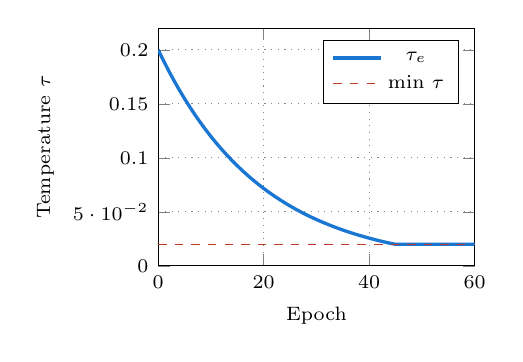
\begin{tikzpicture}
        \begin{axis}[
          width=5.6cm, height=4.6cm,
          xlabel={Epoch}, ylabel={Temperature $\tau$},
          xmin=0, xmax=60, ymin=0, ymax=0.22,
          grid=major, grid style={dotted, neutral},
          label style={font=\scriptsize}, tick label style={font=\scriptsize},
          legend style={font=\scriptsize, at={(0.95,0.95)}, anchor=north east}]
          \addplot[primary, very thick, domain=0:60, samples=61] {max(0.02, 0.2*0.95^x)};
          \addplot[negative, dashed, domain=0:60] {0.02};
          \legend{$\tau_e$, min $\tau$}
        \end{axis}
      \end{tikzpicture}
    \end{column}
  \end{columns}
\end{frame}

\begin{frame}{Training Configuration — Three Variants}
  \centering
  \renewcommand{\arraystretch}{1.18}
  \footnotesize
  \begin{tabular}{lccc}
    \toprule
    \textbf{Hyperparameter} & \textbf{Base THGNN} & \textbf{Hybrid BiGRU} & \textbf{Mamba--MoE} \\
    \midrule
    Hidden / embed dim ($d_h$ / $D$) & 128 & 64 & 64 \\
    GAT heads                        & 4   & 8  & 8 \\
    MAGE layers / MoE experts / MHA heads & --- & 1 / 4 / 2 & 1 / 4 / 2 \\
    Hyperedges (GPH / TCH)           & --- & 32 / 32 & 32 / 32 \\
    Learning rate (peak)             & $1{\times}10^{-4}$ & $2{\times}10^{-4}$ & $1{\times}10^{-4}$ \\
    MSE / IC / Disp weights          & 0.7 / 0.5 / 0.6 & 0.4 / 0.8 / 0.1 & 0.6 / 0.6 / 0.1 \\
    IC warmup (epochs)               & 5 & 5 & 10 \\
    \midrule
    Trainable parameters             & --- & 172{,}637 & --- \\
    Time / epoch (RTX 3050 6\,GB)    & ${\sim}23$\,s & ${\sim}160$\,s & ${\sim}200$\,s \\
    \bottomrule
  \end{tabular}

  \vspace{0.3cm}
  \footnotesize
  Optimizer AdamW, gradient clip $\|\nabla\|_2{\le}1.0$, three-phase LR schedule
  (5-epoch warmup $\rightarrow$ 20-epoch plateau $\rightarrow$ cosine decay).
  \textbf{Splits:} train 2015--2022 \textbar\ val 2023 \textbar\ holdout 2024--2026.
\end{frame}

% ============================================================
\section{Results}
% ============================================================

\begin{frame}{Quantitative Results — Holdout Rank-IC}
  \begin{columns}[T]
    \begin{column}{0.52\textwidth}
      \centering
      \renewcommand{\arraystretch}{1.3}
      \footnotesize
      \begin{tabular}{lcccc}
        \toprule
        \textbf{Model} & \textbf{Epoch} & \textbf{Rank-IC} & \textbf{MSE} & \textbf{Dir-Acc} \\
        \midrule
        Base THGNN   & 2  & 0.0204 & 1.3214 & 48.7\% \\
        Mamba--MoE   & 60 & 0.0343 & 1.2560 & \best{50.8\%} \\
        Hybrid BiGRU & 65 & \best{0.0398} & \best{1.1094} & 50.4\% \\
        \bottomrule
      \end{tabular}

      \medskip
      \footnotesize
      \begin{itemize}\setlength{\itemsep}{3pt}
        \item Hybrid BiGRU: \best{+95.1\%} rank-IC over baseline, $-16\%$ MSE
        \item All three IC estimates statistically significant ($t\!\approx\!9$--$17$, $p<10^{-4}$)
        \item IC $0.02$--$0.04$ matches published US/China results (MASTER: $0.025$--$0.060$)
      \end{itemize}
    \end{column}
    \begin{column}{0.46\textwidth}
      \centering
      
\includegraphics[width=\textwidth]{ic_autocorrelation.png}\\
      \footnotesize Daily IC autocorrelation — all lags within the 95\%
      Bartlett band, validating the i.i.d.\ assumption behind the standard errors.
    \end{column}
  \end{columns}
\end{frame}

\begin{frame}{Holdout Backtest — Four Views}
  \centering
  
\includegraphics[width=\textwidth, height=0.74\textheight, keepaspectratio]{comparison_combined.png}

  \vspace{0.1cm}
  \footnotesize
  Equal-weight dollar-neutral long--short (top-5 $-$ bottom-5), 583 trading days.
  Both hybrids \alert{persistently outperform} the baseline; their 60-day rolling IC
  stays positive while the THGNN's collapses toward zero by 2026.
\end{frame}

\begin{frame}{Backtest Summary \& Quintile Spread}
  \begin{columns}[T]
    \begin{column}{0.50\textwidth}
      \centering
      \renewcommand{\arraystretch}{1.3}
      \footnotesize
      \begin{tabular}{lcccc}
        \toprule
        \textbf{Model} & \textbf{IC} & \textbf{ICIR} & \textbf{Sharpe} & \textbf{MaxDD} \\
        \midrule
        Base THGNN   & 0.0189 & 0.206 & 2.30 & $-0.09$ \\
        Mamba--MoE   & 0.0333 & 0.370 & \best{4.57} & $-0.09$ \\
        Hybrid BiGRU & \best{0.0395} & \best{0.420} & 3.71 & $-0.10$ \\
        \bottomrule
      \end{tabular}

      \medskip
      \footnotesize
      \begin{itemize}\setlength{\itemsep}{3pt}
        \item Hybrid BiGRU: highest, \alert{most consistent} signal (ICIR 0.420)
        \item Only the BiGRU reaches a \alert{negative Q5 return} ($-10.4\%$) —
              genuine \emph{short-side} discrimination
        \item Mamba--MoE: best Sharpe via strongest short-leg mean
      \end{itemize}
    \end{column}
    \begin{column}{0.48\textwidth}
      \centering
      
\includegraphics[width=\textwidth]{comparison_quintile_returns.png}\\
      \footnotesize Monotone Q1$\rightarrow$Q5 decline validates cross-sectional
      discriminative power across the full return distribution.
    \end{column}
  \end{columns}
\end{frame}

\begin{frame}{Return Distribution \& Decile Validation}
  \begin{columns}[c]
    \begin{column}{0.5\textwidth}
      \centering
      
\includegraphics[width=\textwidth]{return_dispersion.png}\\
      \footnotesize Long picks right-shifted vs.\ short. Mamba--MoE has the
      strongest short-leg mean ($-0.309\%$) — its Sharpe premium.
    \end{column}
    \begin{column}{0.5\textwidth}
      \centering
      
\includegraphics[width=\textwidth]{predicted_rank_vs_return.png}\\
      \footnotesize Monotone decile spread; both hybrids yield negative
      bottom-decile returns (slopes: BiGRU 0.018, Mamba 0.017, THGNN 0.013).
    \end{column}
  \end{columns}
\end{frame}

\begin{frame}{Ensemble Agreement as a Confidence Filter}
  \begin{columns}[c]
    \begin{column}{0.62\textwidth}
      \centering
      
\includegraphics[width=\textwidth]{hit_rate_by_agreement.png}
    \end{column}
    \begin{column}{0.36\textwidth}
      \footnotesize
      \textbf{Consensus pays:}
      \begin{itemize}\setlength{\itemsep}{3pt}
        \item 1 model picks: $50\%$ win, $+0.22\%$
        \item 2 models agree: $+0.37\%$
        \item \alert{All 3 agree: $60\%$ win, $+0.83\%$} — nearly 4$\times$ the single-model average
      \end{itemize}
      \smallskip
      Variants capture \alert{partially independent signals} — directly motivating the
      ensemble / stacking direction in future work.
    \end{column}
  \end{columns}
\end{frame}

\begin{frame}{Cost Realism — Turnover \& Breakeven}
  \begin{columns}[c]
    \begin{column}{0.5\textwidth}
      \centering
      
\includegraphics[width=\textwidth]{portfolio_turnover.png}\\
      \footnotesize \textbf{High turnover is structural}: all models replace
      $89$--$93\%$ of their top-5 book daily — near-full round-trip costs each day.
    \end{column}
    \begin{column}{0.5\textwidth}
      \centering
      
\includegraphics[width=\textwidth]{cost_adjusted_sharpe.png}\\
      \footnotesize Sharpe breakeven costs: THGNN ${\approx}10$\,bp,
      BiGRU ${\approx}22$\,bp, \alert{Mamba--MoE ${\approx}28$\,bp} (most cost-robust).
    \end{column}
  \end{columns}
  \smallskip
  \centering\footnotesize
  At a representative Indian round-trip cost of ${\sim}15$\,bp the baseline turns
  unprofitable, while \alert{both hybrids retain positive net Sharpe}.
\end{frame}

\begin{frame}{Learning Dynamics — Hybrid Variants}
  \begin{columns}[c]
    \begin{column}{0.5\textwidth}
      \centering
      
\includegraphics[width=\textwidth]{2023-12-29_hybrid_loss_curve.png}\\
      \footnotesize \textbf{Hybrid BiGRU}: healthy convergence; rank-IC grows
      monotonically to 0.040 at epoch 65, no overfitting.
    \end{column}
    \begin{column}{0.5\textwidth}
      \centering
      
\includegraphics[width=\textwidth]{2023-12-29_mamba_moe_loss_curve.png}\\
      \footnotesize \textbf{Mamba--MoE}: validation loss plateaus from epoch 50;
      IC-patience termination at epoch 85.
    \end{column}
  \end{columns}
  \smallskip
  \centering\footnotesize
  Both hybrids exploit the \alert{temperature-annealed soft-rank objective} to sharpen
  cross-sectional ranking as training matures.
\end{frame}

\begin{frame}{Learning Dynamics — Baseline Saturation}
  \begin{columns}[c]
    \begin{column}{0.5\textwidth}
      \centering
      
\includegraphics[width=\textwidth]{2023-12-29_thgnn_loss_curve.png}\\
      \footnotesize \textbf{Base THGNN}: composite loss; early stopping triggers
      at epoch 22, best checkpoint saved at epoch 2.
    \end{column}
    \begin{column}{0.5\textwidth}
      \centering
      
\includegraphics[width=\textwidth]{2023-12-29_thgnn_rank_ic_curve.png}\\
      \footnotesize \textbf{Base THGNN rank-IC}: saturates at epoch 2 then
      oscillates around 0.020 — the architecture's ceiling under its loss regime.
    \end{column}
  \end{columns}
  \smallskip
  \centering\footnotesize
  The simpler GRU–3-stream-GAT exhausts its representational capacity within a few
  gradient passes — \alert{saturation, not instability}.
\end{frame}

% ============================================================
\section{Multi-Agent Decision Pipeline}
% ============================================================

\begin{frame}{Six-Agent LangGraph Pipeline}
  \centering
  
\includegraphics[width=\textwidth, height=0.55\textheight, keepaspectratio]{multiagent_pipeline.png}

  \vspace{0.1cm}
  \footnotesize
  \begin{columns}[T]
    \begin{column}{0.5\textwidth}
      \textbf{1. GNN} — trained checkpoint $\rightarrow$ score vector $\hat{\myvec{y}}$\\
      \textbf{2. News} — FinBERT sentiment $s_i\in[-1,1]$ per stock\\
      \textbf{3. Portfolio} — fuse: $\text{score}_i=\alpha\,\text{rank}(\hat y_i)+(1{-}\alpha)\,\text{norm}(s_i)$
    \end{column}
    \begin{column}{0.5\textwidth}
      \textbf{4. Risk} — beta, vol, 52-wk range, ATR $\rightarrow$ L/M/H label\\
      \textbf{5. Macro} — NIFTY trend + India VIX $\rightarrow$ regime multiplier $c$\\
      \textbf{6. Report} — Google \texttt{gemma-4-31b} $\rightarrow$ research note
    \end{column}
  \end{columns}
  \smallskip
  \centering Sentiment is fused at the \alert{portfolio level} — $\alpha$ is tunable at inference without retraining.
\end{frame}

\begin{frame}{Live Run — 25 May 2026 (Hybrid BiGRU, $\alpha{=}0.60$)}
  \begin{columns}[T]
    \begin{column}{0.52\textwidth}
      \centering
      \renewcommand{\arraystretch}{1.15}
      \scriptsize
      \begin{tabular}{lccc c}
        \toprule
        \textbf{Ticker} & \textbf{Action} & \textbf{GNN} & \textbf{Sent.} & \textbf{Fusion} \\
        \midrule
        JUBLPHARMA & \textcolor{positive}{\textbf{BUY}}  & 1.000 & ---    & 1.000 \\
        EIDPARRY   & \textcolor{positive}{\textbf{BUY}}  & 0.900 & ---    & 0.900 \\
        DEEPAKNTR  & \textcolor{positive}{\textbf{BUY}}  & 0.950 & $+0.93$ & 0.869 \\
        \midrule
        INDIGO     & \textcolor{negative}{\textbf{SELL}} & 0.650 & $-0.07$ & 0.446 \\
        RHIM       & \textcolor{negative}{\textbf{SELL}} & 0.200 & $+0.93$ & 0.420 \\
        ERIS       & \textcolor{negative}{\textbf{SELL}} & 0.050 & $+0.94$ & 0.331 \\
        \bottomrule
      \end{tabular}

      \medskip
      \footnotesize
      \begin{itemize}\setlength{\itemsep}{2pt}
        \item GNN \alert{dominates} SELL leg even when sentiment is positive
              (RHIM: low rank $\rightarrow$ SELL)
        \item Negative sentiment correctly integrated (INDIGO — crude-oil headwinds)
        \item End-to-end latency ${\approx}47$\,s (incl.\ LLM report)
      \end{itemize}
    \end{column}
    \begin{column}{0.46\textwidth}
      \centering
      
\includegraphics[width=\textwidth]{streamlit_demo.png}\\
      \footnotesize Streamlit live portfolio tab: macro regime banner
      (BULL, VIX 16.7, conviction $1.00\times$) above the ranked allocation table.
    \end{column}
  \end{columns}
\end{frame}

\begin{frame}{Fusion-Weight Sensitivity ($\alpha$ Sweep)}
  \begin{columns}[T]
    \begin{column}{0.55\textwidth}
      \centering
      \renewcommand{\arraystretch}{1.25}
      \footnotesize
      \begin{tabular}{ccccc}
        \toprule
        $\alpha$ & GNN & Sent. & $\rho$ vs GNN & SELL $\Delta$ \\
        \midrule
        0.0 & 0\%   & 100\% & $-0.094$ & 4 \\
        0.3 & 30\%  & 70\%  & $+0.634$ & 4 \\
        0.5 & 50\%  & 50\%  & $+0.795$ & 3 \\
        0.7 & 70\%  & 30\%  & $+0.979$ & 1 \\
        1.0 & 100\% & 0\%   & $+1.000$ & 0 \\
        \bottomrule
      \end{tabular}
    \end{column}
    \begin{column}{0.43\textwidth}
      \footnotesize
      \textbf{Three findings:}
      \begin{enumerate}\setlength{\itemsep}{4pt}
        \item BUY set is \alert{entirely stable} from $\alpha{=}0.3$ to $1.0$
        \item SELL set is more sensitive — sentiment can \emph{rescue} a
              borderline short with strong fundamental news
        \item At $\alpha{=}0.7$, $\rho{=}0.979$ with pure GNN — predictions
              dominate, sentiment provides \alert{targeted overrides}
      \end{enumerate}
      \smallskip
      Illustrative (single session, $N{=}21$); a multi-day sweep is future work.
    \end{column}
  \end{columns}
\end{frame}

% ============================================================
\section{Conclusion}
% ============================================================

\begin{frame}{Key Findings}
  \begin{columns}[T]
    \begin{column}{0.5\textwidth}
      \begin{block}{What worked}
        \begin{itemize}\setlength{\itemsep}{3pt}
          \item \textbf{Dual-hypergraph + MAGE} is the primary driver of the
                rank-IC gain (causal masking + latent group learning)
          \item \textbf{Composite IC loss} drives sustained improvement —
                IC grows to epoch 65 vs.\ saturation at epoch 2 for baseline
          \item \textbf{Ensemble consensus} carries 4$\times$ the expected return
        \end{itemize}
      \end{block}
    \end{column}
    \begin{column}{0.5\textwidth}
      \begin{block}{Trade-offs}
        \begin{itemize}\setlength{\itemsep}{3pt}
          \item \textbf{BiGRU} wins on rank-IC \& ICIR $\Rightarrow$ best for
                \emph{ranking} strategies
          \item \textbf{Mamba--MoE} wins on directional accuracy, Sharpe \&
                cost-robustness $\Rightarrow$ best for \emph{directional} signals
          \item Indian equity forecasting is \emph{tractable but hard} —
                IC $0.02$--$0.04$ is on par with US/China benchmarks
        \end{itemize}
      \end{block}
    \end{column}
  \end{columns}
\end{frame}

\begin{frame}{Limitations \& Future Work}
  \begin{columns}[T]
    \begin{column}{0.48\textwidth}
      \textbf{Limitations}
      \begin{itemize}\setlength{\itemsep}{3pt}
        \item \alert{Transaction costs}: $89$--$93\%$ daily turnover; baseline
              unprofitable above ${\sim}15$\,bp
        \item Fixed temporal split — no walk-forward re-training
        \item Single-day horizon only
        \item \alert{No component-level ablation} — the $+95\%$ gain blends
              architecture and loss-regime changes
        \item Inputs limited to price/volume; sentiment fused only at portfolio layer
      \end{itemize}
    \end{column}
    \begin{column}{0.48\textwidth}
      \textbf{Future work}
      \begin{enumerate}\setlength{\itemsep}{3pt}
        \item \alert{Loss-weight ablation} (highest priority) — grid / Bayesian search
        \item Walk-forward backtest with monthly retraining
        \item End-to-end sentiment fusion into the GNN tensor
        \item \alert{BiGRU + Mamba ensemble} — complementary IC \& direction profiles
        \item Multi-horizon prediction (1 / 5 / 20-day)
        \item Cross-market generalisation (BSE 500, Nikkei, Hang Seng)
      \end{enumerate}
    \end{column}
  \end{columns}
\end{frame}

\begin{frame}[standout]
  Thank you
  \vspace{0.4cm}

  {\large Graph-Structured Deep Learning for Financial Forecasting}

  \vspace{0.2cm}
  {\normalsize Hybrid THGNN--MaGNet \;\textbar\; rank-IC \best{0.0398} (+95\%) \;\textbar\; NIFTY 500}

  \vspace{0.6cm}
  {\small Debarshi Chakraborty \quad Questions?}
\end{frame}

% ---- Appendix -----------------------------------------------
\appendix

\begin{frame}{References}
  \footnotesize
  \begin{thebibliography}{9}
    \bibitem{thgnn} Xiang et al.\ (2022). \textit{Temporal and Heterogeneous Graph
      Neural Network for Financial Time Series Prediction.} CIKM.
    \bibitem{magnet} \textit{MaGNet: Mamba Dual-Hypergraph Network for Stock Prediction.}
    \bibitem{mamba} Gu \& Dao (2023). \textit{Mamba: Linear-Time Sequence Modeling
      with Selective State Spaces.}
    \bibitem{master} Li et al.\ (2024). \textit{MASTER: Market-Guided Stock Transformer.} AAAI.
    \bibitem{sthan} Sawhney et al.\ (2021). \textit{Stock Selection via Spatiotemporal
      Hypergraph Attention Network.} AAAI.
    \bibitem{pairnorm} Zhao \& Akoglu (2020). \textit{PairNorm: Tackling Oversmoothing
      in GNNs.} ICLR.
    \bibitem{finbert} Araci (2019). \textit{FinBERT: Financial Sentiment Analysis with
      Pre-trained Language Models.}
  \end{thebibliography}
\end{frame}

\end{document}
